% % % % % % % % % % % % % % % % % % % % % % % % % % % % % % % % % % % % % % % % 
% LaTeX4EI Example for Cheat Sheets									
%
% @encode: 	UTF-8, tabwidth = 4, newline = LF
% @author:	LaTeX4EI		
% % % % % % % % % % % % % % % % % % % % % % % % % % % % % % % % % % % % % % % % 


% ======================================================================
% Document Settings
% ======================================================================

% possible options: color/nocolor, english/german, threecolumn
% default: color, english
\documentclass[german]{latex4ei/latex4ei_sheet}

\usepackage{multirow}

% set document information
\title{Mathematik}
\author{LaTeX4EI}					% optional, delete if unchanged
\myemail{info@latex4ei.de}			% optional, delete if unchanged

\DeclareMathOperator{\cond}{cond}
\DeclareMathOperator{\rang}{rang}

\DeclareMathOperator{\Bild}{Bild}
\DeclareMathOperator{\defect}{def}

\renewcommand{\i}{\ensuremath{\boldsymbol{\mathrm{i}}}}

% DOCUMENT_BEGIN ===============================================================
\begin{document}

\maketitle	% requires ./img/Logo.pdf

% SECTION ====================================================================================
\section{Temporal Tests}
% ============================================================================================

$\ma A \in \R^2: \det \ma A \widehat = $ Fläche Parallelogram!\\
$\ma A \in \R^3: \det \ma A \widehat = $ Volumen Spat.!\\


\begin{sectionbox}
	\subsection{Mengen}
	Eine Zusammenfassung wohlunterschiedener Elemente zu einem Ganzen.
	Explizite Angabe: $A=\{1;2;3\}$\\
	Angabe durch Eigenschaft: $A=\{n\in \N\ \vert\ 0<n<4\}$\\

	\subsubsection{Mengenregeln}
	\begin{tablebox}{lll}
		%& $(P(\Omega);\capdot , \cupplus, \overline{A};\Omega,\emptyset )$\\ \mrule
		Kommutativ 		& $A \capdot B = B \capdot A$ & $A \cupplus B = B \cupplus A$\\
		Assoziativ 		& \multicolumn{2}{l}{ $(A \capdot B) \capdot C = A \capdot (B \capdot C)$} \\
						& \multicolumn{2}{l}{$(A \cupplus B) \cupplus C = A \cupplus (B \cupplus C)$} \\
		Distributiv 	& \multicolumn{2}{l}{$A \capdot (B \cupplus C) = (A \capdot B) \cupplus (A \capdot C)$}\\
						& \multicolumn{2}{l}{ $A \cupplus (B \capdot C) = (A \cupplus B) \capdot (A \cupplus C)$}\\ \cmrule
		Indempotenz		& $A \capdot A = A$ & $A \cupplus A = A$\\
		Absorbtion		& $A \capdot (A \cupplus B) = A$ & $A \cupplus (A \capdot B) = A$\\
		Neutralität		& $A \capdot \Omega = A$ & $A \cupplus \emptyset = A$\\
		Dominant		& $A \capdot \emptyset = \emptyset$ & $A \cupplus \Omega = \Omega$\\
		Komplement		& $A \capdot \overline{A} = \emptyset$ & $A \cupplus \overline{A} = \Omega$\\
						& $\overline{\overline{A}} = A$ & $\ol{\Omega} = \emptyset$\\
		De Morgan		& $\overline{A \capdot B} = \overline{A} \cupplus \overline{B}$ & $\overline{A \cupplus B} = \overline{A} \capdot \overline{B}$\\
	\end{tablebox} 


	\subsubsection{Wichtige Mengen}
	\begin{tablebox}{rll}
		$\emptyset$ & $=\{ \}$ & Leere Menge\\
		$\mathbb N$ & $=\{1,2,3,4,5,\dotsc\}$ & Natürliche Zahlen \\
		$\mathbb Z$ & $=\{\dotsc ,-2,-1,0,1,2,\dotsc\}$ & Ganze Zahlen \\
		$\mathbb Q$ & $=\iset {\frac m n}{  m \in \mathbb Z, n \in \mathbb N }$ & Rationale Zahlen\\
		$\mathbb R$ & $=\{\dotsc ,-\sqrt{2},\dotsc,0,\dotsc,\pi,\dotsc\}$ & Reele Zahlen\\	
		$\mathbb C$ & $=\mathbb R^2$ & Komplexe Zahlen\\
		$\mathbb B$ & $=\{ 0,1 \}$ & Binäre Zahlen\\		
		$\mathbb S$ & $=\{ -1,0,1 \}$ & Vorzeichenmenge\\	
		$\mathcal K[x]$ & & Polynomring\\ 		
	\end{tablebox}
\end{sectionbox}


\begin{sectionbox}
	\subsection{Vollständige Induktion}
	Behauptung: $f(n)=g(n)$ für $n_0 \le n \in \mathbb N$\\ 
	IA: $n=n_0$: \quad Zeige $f(n_0)=g(n_0)=$wahr.\\
	IV: Behauptung gilt für ein beliebiges $n\in\mathbb N$ \quad (Sei $f(n)=$wahr)\\
	IS: $n \rightarrow n+1$: \quad Zeige $f(n+1)=\underset{=wahr}{f(n)}  \dotsc=g(n+1)$
\end{sectionbox}

\begin{sectionbox}
	\subsection*{Binome, Trinome}
	$(a\pm b)^2 = a^2 \pm 2ab + b^2$ \hfill $a^2 - b^2 = (a-b)(a+b)$\\
	$(a \pm b)^3 = a^3 \pm 3a^2b + 3ab^2 \pm b^3$\\
	$(a+b+c)^2 = a^2 + b^2 + c^2 + 2ab + 2ac + 2bc$
\end{sectionbox}


\begin{sectionbox}
	\subsection{Mittelwerte \quad $\min x_i \le \ol x_{\ir{harm}} \le \ol x_{\ir{geo}} \le \ol x_{\ir{ar}} \le \max x_i$}
	\begin{tablebox}{lll} 
	\textbf{Arithmetisches} & $\ge$ \textbf{Geometrisches} & $\ge$ \textbf{Harmonisches}\\ \cmrule
	$\ol x_{\ir{ar}} = \frac{1}{N} \sum\limits^N_{i = 1} x_i$ & $\ol x_{\ir{geo}} = \sqrt[N]{ \prod\limits^N_{i = 1} x_i }$ & $\ol x_{\ir{hm}} =$\raisebox{0.5em}{ $\frac{N}{\sum\limits^N_{i = 1} \frac{1}{x_i}}$}\\ 
	\end{tablebox}
	Median: Zahl in der Mitte einer geordneten(ordinalen) Liste.\\
	Modalwert: Häufigster Wert (geht auch bei nominaler Liste).
\end{sectionbox}



\subsection{Komplexe Zahlen $a + b\i = \cx z \in \C = \R^2$}
% ----------------------------------------------------------------------
$\cx z$ mit Realteil $\Re{\cx z}=a \in \R$ und Imaginärteil $\Im{\cx z}=b \in \R$\\
\parbox{2cm}{ 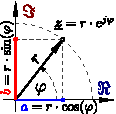
\includegraphics{./img/trigo.pdf} } \quad
\parbox{6cm}{ 
	$\cx z = \underset{\text{Karthesisch}}{a + b\i} = \underset{\text{Polarkoord.}}{r \cdot e^{\i \varphi}}$ \quad\ \boxed{ \underset{\text{Imaginäre Einheit}}{\i = \sqrt{-1}}}\\[0.4em] 
	$\i^{2n} = -1^n$ \quad\ $\i^{2n+1} = -\i^n$ \quad\ $\i^{-1} = -\i$ \\[0.2em] 
	Konjugiert: $\ol{\cx z} = a - b\i$ \qquad $e^{\overline{iφ}} = e^{-iφ}$ \\ $\cx z \ol{\cx z} = \abs{\cx z}^2 = a^2+b^2$\\[0.2em]
	$\cx z_1 \cdot \cx z_2 = r_1 \cdot r_2 \cdot e^{\i (\varphi_1 + \varphi_2)}$\\[0.2em]
	Inverse $z^{-1} = \frac{\ol{\cx z}}{\ol{\cx z} \cx z}=\frac{a - b\i}{a^2+b^2}$ }


Es gilt: \quad $i^2 = -1$ \quad $i^4 = 1$
\subsubsection{Kartesische Koordinaten}
Rechenregeln:\\
$z_1+z_2=(a_1+a_2)+(b_1+b_2)\mathbf{i}$\\
$z_1\cdot z_2=(a_1\cdot a_2-b_1\cdot b_2)+(a_1\cdot b_2+a_2\cdot b_1)\mathbf{i}$\\


\subsubsection{Polarkoordinaten}
$z=a+b\mathbf{i}\ne0$\ in Polarkoordinaten:\\
$z=r (\cos(\varphi)+\mathbf{i}\sin(\varphi))=r\cdot e^{\varphi \mathbf{i}}$\\
$r=|z|=\sqrt{a^2+b^2}\quad\varphi=\arg(z)=\begin{cases}+\arccos \left( \frac{a}{r}\right),  & b\ge0   \\  -\arccos \left( \frac{a}{r}\right), & b<0\end{cases}$

\begin{description}\itemsep0pt
\item[Multiplikation:] $z_1\cdot z_2=r_1 * r_2 ( \cos ( \varphi_1 + \varphi_2) + \mathbf{i} \sin (\varphi_1 + \varphi_2))$
\item[Division:] $\frac{z_1}{z_2}=\frac{r_1}{r_2} ( \cos ( \varphi_1 - \varphi_2) + \mathbf{i} \sin (\varphi_1 - \varphi_2))$
\item[n-te Potenz:] $z^n=r^n\cdot e^{n\varphi \mathbf{i}}= r^n (\cos (n \varphi) + \mathbf{i} \sin (n \varphi))$
\item[n-te Wurzel:] $\sqrt[n]{z}= z_k = \sqrt[n]{r} \left(\cos \left(\frac{\varphi + 2k\pi}{n}\right) + \mathbf{i} \sin \left(\frac{\varphi + 2k\pi}{n}\right)\right) \\ k =0,1, \ldots, n-1$
\item[Logarithmus:] $\ln(z)=\ln(r) + \mathbf{i}(\varphi + 2k\pi)$ \quad (Nicht eindeutig!)
\end{description}
Anmerkung: Addition in kartesische Koordinaten umrechnen(leichter)!


\begin{sectionbox}
	\subsection{Exponentialfunkt. und Logarithmus\ \ $e = 2,718281828$}
	$\exp(x) \equiv e^x := \lim\limits_{n \rightarrow \infty} \left( 1 + \frac{x}{n} \right)^n = \sum\limits_{n = 0}^{\infty} \frac{x^n}{n!}$\\
	\begin{tabular*}{\columnwidth}{l@{\extracolsep\fill}ll}
		$a^x = e^{x \ln a}$ & $\log_a x = \frac{\ln x}{\ln a}$ & $\ln x \le x -1$\\
		$\ln(x^{a}) = a \ln(x)$ & $\ln(\frac{x}{a}) = \ln x - \ln a$ & $\log(1) = 0$\\
	\end{tabular*}
\end{sectionbox}




\begin{sectionbox}
	Folge (Sequenz) definiert durch Funktion, Reihe, Rekursion\\

	\subsection{Reihen}
	$\underset{\text{Harmonische Reihe}}{\sum\limits_{n=1}^\infty \frac{1}{n} \ra \infty} \qquad\qquad   \underset{\text{Geometrische Reihe}}{\sum\limits_{n=0}^\infty q^n \stackrel{|q|<1}= \frac{1}{1-q}}  \qquad\qquad \underset{\text{Exponentialreihe}}{\sum\limits_{n = 0}^{\infty} \frac{\cx z^n}{n!} = e^{\cx z}}$\\[0.5em]
	$\sum\limits_{n = 0}^{\infty} (-1)^n \frac{z^{2n +1}}{(2n +1)!} = \sin(z) \qquad \sum\limits_{n = 0}^{\infty} (-1)^n \frac{z^{2n}}{(2n)!} = \cos(z)$\\

	\subsubsection{Taylorpolynom $T_{m,f,x_0}(x)$ (Reihe für $m \ra \infty$)}
	\boxed{ T(x)= \sum_{i=0}^{m}  \underbrace{\frac{f^{(i)}(x_0)}{i!}}_{a_i} (x-x_0)^i } \ \parbox{3.0cm}{ Konvergenzradius \\ $R=\underset{i\rightarrow \infty}{\lim} \abs{\frac{a_i}{a_{i+1}}}$ }\\
\end{sectionbox}


% SECTION ====================================================================================
\section[Abbildungen]{Abbildungen $\vec f:\mathbb D^n \rightarrow \mathbb W^m,\ \vec x \mapsto \vec f(\vec x)$ }
% ============================================================================================

\begin{sectionbox}
	% Vielleicht: kleines Graphenbild zur Vernaschaulichung?
	\fbox{ \everymath{\displaystyle}
	\begin{tabular}{rl|rl}
		Funktion & $f:\mathbb D \rightarrow \mathbb W$ & Skalarfeld & $\phi:\mathbb D^n \rightarrow \mathbb W$ \\ \mrule
		Kurve & $\vec r: \mathbb D \rightarrow \mathbb W^m$ & Vektorfeld & $\vec F:\mathbb D^n \rightarrow \mathbb W^n$ \\ \mrule
		\multicolumn{4}{c}{Vektorwertige Funktion $\vec f:\mathbb D^n \rightarrow \mathbb W^m$} \\
	\end{tabular} \everymath{\textstyle} }
	
	\begin{tabular*}{\columnwidth}{@{\extracolsep\fill}ll@{}}
	\textbf{Bild} $f(D) := \iset{f(x)}{x\in D}$ & \textbf{Kern} $\ker f := \iset{\vec x}{\vec f(\vec x) = \vec 0}$   \\
	\textbf{Komposition} $f \circ g := f\bigl( g(x) \bigr)$ & \textbf{Fixpunkt} $a := f(a)$ \\
	\end{tabular*} 
	
	\begin{tabular}{@{}lll}
			\textbf{Injektiv} & $f(x_1)=f(x_2) \Rightarrow x_1=x_2$ & \multirow{2}{2.0cm}{\Big \} beides: \textbf{Bijektiv} }\\
			\textbf{Surjektiv} & $\forall y\in \mathbb W \exists x\in \mathbb D:f(x)=y$ & \\ 
	\end{tabular}\\ 
\end{sectionbox}

\begin{sectionbox}
	\subsection{Funktionen $f:\mathbb D \rightarrow \mathbb W,\ x \mapsto f(x)$}
	Eine Funktion $f$ ist eine Abbildung, die jedem Element $x$ einer Definitionsmenge $D$ genau ein Element $y$ einer Wertemenge $W$ zuordnet.
	%===========================================================================================================================================================
	\textbf{Achsensym.}($g$): $f(-x)=f(x)$ \qquad \textbf{Punktsym.}($u$): $f(-x)=-f(x)$\\
	\begin{tabular}{@{}lll}
	$g_1 \pm g_2 = g_3$ & \quad $u_1 \pm u_2 = u_3$ & \quad gerade/ungerade Fkt. $g/u$\\
	$g_1 \cdot g_2=g_3$ & \quad $u_1 \cdot u_2 = g_3$ & \quad $u_1 \cdot g_1=u_3$
	\end{tabular}

			\subsubsection{Extrema, Monotonie und Krümmung von $f$}
			$f'(x_0)\overset{!}{=}0 \quad \begin{cases}f''(x_0)<0 \ \rightarrow \ \text{Maximum (lokal)} \\ f''(x_0)>0 \ \rightarrow \ \text{Minimum (lokal)}\end{cases} $\\
			$f''(x_0)=0 \text{ und } f'''(x_0) \ne 0 \rightarrow x_0$ Wendepunkt \\
			$f'(x) \stackrel{_\ge}{_{(>)}}\!\! / \!\! \stackrel{_\le}{_{(<)}} 0 \ \rightarrow$ \ $f$ (streng) Monoton steigend/fallend. $x\in[a,b]$\\
			$f''(x) \stackrel{_\ge}{_{(>)}}\!\! / \!\! \stackrel{_\le}{_{(<)}} 0 \ \rightarrow$ \ $f$ (strikt) konvex/konkav. $x\in[a,b]$\\
\end{sectionbox}

\begin{sectionbox}
	\subsection{Asymptoten und Grenzwerte von $f$}
	Horizontal: $c_\pm =\lim\limits_{x\ra \pm \infty} f(x)$ \qquad Vertikal: $\exists\,\text{Nullst. } a \text{ des Nenners }$\\ %: \lim\limits_{x \rightarrow a^{\pm}} f(x) = \pm \infty$\\
	Polynomasymptote $P(x)$: $f(x):=\frac{A(x)}{Q(x)}=P(x)+ \Big(\frac{B(x)}{Q(x)}\ra 0\Big)$\\
	\textbf{Regel von L'Hospital}: $\lim\limits_{x \rightarrow a} \frac{f(x)}{g(x)} \rightarrow \left[ \frac{0}{0} \right]\!/\!\left[ \frac{\infty}{\infty} \right] = \lim\limits_{x \rightarrow a} \frac{f'(x)}{g'(x)}$\\[0.5em]

		\subsubsection{Wichtige Grenzwerte}
		\begin{tabular*}{\columnwidth}{l@{\extracolsep\fill}ll}
			$\lim\limits_{x \ra \infty} \frac{1}{x^n} = 0$ & $\lim\limits_{n \ra \infty} \sqrt[n]{n} = 1$ & $\lim\limits_{n \ra \infty} \frac{n^n}{n!} = \infty$\\
			$\lim\limits_{x \ra \infty} x \cdot e^{-x} = 0$ & $\lim\limits_{x \ra 0} \frac{\sin(x)}{x} = 1$ & $\lim\limits_{x \ra 0} \frac{x}{\sin(x)} = 1$\\
		\end{tabular*}

		\subsubsection{Wichtige Sätze für \emph{stetige} Fkt. $f: [a,b] \rightarrow \mathbb R, f \mapsto f(x)$ }
		\textbf{Zwischenwertsatz:} $\forall y \in [f(a),f(b)]\ \exists x\in [a,b]:f(x)=y$\\
		\textbf{Mittelwertsatz:} Falls $f$ diffbar, dann $\exists x_0:f'(x_0)=\frac{f(b)-f(a)}{b-a}$\\
		\textbf{Satz von Rolle:} Falls $f(a)=f(b)$, dann $\exists x_0: f' (x_0) = 0$\\ 
\end{sectionbox}


\begin{sectionbox}
	\subsection{Polynome $P(x)\in\mathbb R[x]_n = \sum\limits_{i=0}^n a_ix^i$ vom Grad $n$}
	\vspace{-0.5em}
	\parbox{3cm}{ 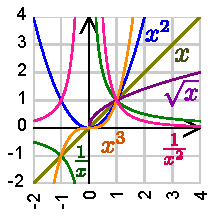
\includegraphics[scale = 0.8]{./img/polynome.pdf}}
	\parbox{3.5cm}{ \textbf{Gerade} durch Punkt $P(x_0,y_0)$:\\[0.2em] $y = m(x - x_0) + y_0$ \\
	\\
	\textbf{Quadratisch:} $y = ax^2+bx+c$\\[0.2em]
	Mitternachtsformel für Nullstellen:\\
	\boxed{ x_{1/2}=\frac{-b\pm\sqrt{b^2-4ac}}{2a} }\\
	$x_1 + x_2 = - \frac{b}{a} \qquad x_1 x_2 = \frac{c}{a}$
	}
\end{sectionbox}




% SECTION ====================================================================================
\section{Trigonometrie}
% ============================================================================================

\begin{sectionbox}
	\subsection[Sinus, Cosinus]{Sinus, Cosinus $\sin^2 x + \cos^2 x = 1$}
	$\sin (-x) = -\sin (x)$  \qquad $\cos (-x) = \cos (x)$ \\
	$e^{\i x}=\cos(x)+\i\sin(x)$, $e^{-\i x}=\sin(x)-\i\cos(x)$
	\begin{tablebox}{c|c|c|c|c||c|c|c|c}
		$x$ & $0$ & $\pi / 6$ & $\pi / 4$ & $\pi / 3$ & $\frac{1}{2}\pi$ & $\pi$ & $1\frac{1}{2}\pi$ & $2 \pi$ \\
		$\scriptstyle{ \varphi }$ & $\scriptstyle{0^\circ}$ & $\scriptstyle{30^\circ}$ & $\scriptstyle{45^\circ}$ & $\scriptstyle{60^\circ}$ & $\scriptstyle{90^\circ}$ & $\scriptstyle{180^\circ}$ & $\scriptstyle{270^\circ}$ & $\scriptstyle{360^\circ}$ \\ \cmrule
		$\sin$ & $0$ & $\frac{1}{2}$ & $\frac{1}{\sqrt{2}}$ & $\frac{\sqrt 3}{2}$ & $1$ & $0$ & $-1$ & $0$ \\
		$\cos$ & $1$ & $\frac{\sqrt 3}{2}$ & $\frac{1}{\sqrt 2}$ & $\frac{1}{2}$ & $0$ & $-1$ & $0$ & $1$ \\     
		$\tan$ & $0$ & $\frac{\sqrt{3}}{3}$ &	$1$	&	$\sqrt{3}$ & $\pm \infty$ & $0$ & $\mp \infty$ & $0$\\ 
	\end{tablebox}
	\begin{tabular*}{\columnwidth}{@{\extracolsep\fill}ll@{}}
		Additionstheoreme &  Stammfunktionen\\
		$\cos (x - \frac{\pi}{2}) = \sin x$ & $\int x \cos(x) \diff x = \cos(x) + x \sin(x)$\\
		$\sin (x + \frac{\pi}{2}) = \cos x$ & $\int x \sin(x) \diff x = \sin(x) - x \cos(x)$\\
		$\sin 2x = 2 \sin x \cos x $  & $\int \sin^2(x) \diff x = \frac12 \bigl(x - \sin(x)\cos(x) \bigr)$\\
		$\cos 2x = 2\cos^2 x - 1$  & $\int \cos^2(x) \diff x = \frac12 \bigl(x + \sin(x)\cos(x) \bigr)$\\
		$\sin(x) = \tan(x)\cos(x)$ & $\int \cos(x)\sin(x) = -\frac12 \cos^2(x)$ \\
	\end{tabular*}\\[1em]
	\textbf{Sinus/Cosinus Hyperbolicus} $\sinh, \cosh$\\
	\begin{tabular*}{\columnwidth}{@{\extracolsep\fill}ll@{}}
		$\sinh x = \frac{1}{2}(e^x -e^{-x})= - \j \, \sin(\j x)$ & $\cosh^2 x  \bs - \sinh^2 x = 1$\\
		$\cosh x  = \frac{1}{2}(e^x +e^{-x})= \cos(\j x)$ & $\cosh x + \sinh x = e^{x}$\\
	\end{tabular*}\\
\end{sectionbox}


\begin{sectionbox}
	\subsection{Kurven $\vec \gamma: [a,b] \ra \R^n, t \mapsto \vec \gamma(t)$}
	%===========================================================================================================================================================
	\textbf{Bogenlänge:} \\ $L(\vec \gamma) = \int\limits_{a}^{b} \norm{\dot {\vec \gamma}(t)} \mathrm dt$ \\[1em] \textbf{Krümmung:}\\ $\kappa(t)= \norm{\frac{\mathrm d^2 \vec \gamma}{\mathrm d s^2}} = \frac{\norm{\dot T(t)}}{s'(t)}$ \\ $s: [a,b] \ra [0,L(\vec \gamma)], t \mapsto s(t)$ \\ (nach Bogenlänge parametr.) 


$\mathcal C^n$-Kurve: $n$-mal stetig diffbar, $\mathcal C^0$-Kurve: geschlossene Kurve\\
regulär, falls $\forall t \in [a,b]:\dot \gamma(t) \ne \vec 0$ (Keine Knicke), sonst singulär
\end{sectionbox}


\begin{sectionbox}
	\subsection{Skalarfelder $φ:\mathbb D \subseteq \R^n \rightarrow \R$}
	%===========================================================================================================================================================
	Richtungsableitung: $\partial_v f(\vec x) =  \nabla f(\vec x)^\top \bdot \vec v$ mit $ \norm{\vec v}=1 $
\end{sectionbox}



% SECTION ====================================================================================
\section{Lineare Algebra}
% ============================================================================================

\begin{sectionbox}
	\subsection{Algebraische Strukturen $S(*)$}
	Menge $S$ mit binären Verknüpfungen $*:S\times S \rightarrow S$, deren Elemente bestimmte Axiome erfüllen ($a,b,c \in S$):
	\begin{itemize}\itemsep0pt
		\item Assoziativ: $(a* b) * c = a * (b * c)$
		\item Neutrales Element: $\forall a \exists_1 e \in S: a * e = e * a = a$ % \quad (meist $0$ oder $1$)
		\item Inverses Element: $\forall a \exists_1 a^{-1} \in S: a * a^{-1} = e$
		\item Kommutativ: $a * b = b * a$
		\item Distributiv: $a \cdot (b+c)=a\cdot b + a \cdot c$		
	\end{itemize}

	\begin{tablebox}{ll}
		Struktur & Definition \\ \cmrule
		Halbgruppe $(S,*)$ & $*$ ist assoziativ \\
		Monoid $(S,*)$ & Halbgruppe mit neutralem Element $e$\\
		Gruppe $(S,*)$ & Monoid mit Inversem $^{-1}$\\
		Abelsche Gruppe $(S,*)$ & Gruppe, so dass $*$ kommutativ ist.\\
		Ring $(S,+,\cdot)$ & abelsche Gruppe $(S,+)$, \\ & Halbgruppe $(S,\cdot)$, Distributivgesetz \\
		Körper $(S,+,\cdot)$ & Ring mit abelscher Gruppe $(S\setminus\{ 0 \}, \cdot)$\\
	\end{tablebox}
\end{sectionbox}


\begin{sectionbox}
	\subsection[Vektorräume]{Vektorräume $V$}
	$(V,+,\bdot)$ is K-Vektorraum über Körper $(\K,+,\cdot)$. Es gilt: $\vec v \in \K^n$\\
	\textbf{Linear Unabhängig:} Vektoren heißen linear unabhängig, wenn aus: \\
	$\alpha_1 \vec v_1 + \alpha_2 \vec v_2 + \ldots + \alpha_n \vec v_n = \vec 0$ folgt, dass alle $\alpha_i = 0$\\
	\textbf{Basis} $\ma B=\eset{\vec b_1, \vec b_2, ...}$: $n$ Vektoren, linear unabhängig, erzeugen $V$\\
	\textbf{Betrag (Norm):} $\norm{\vec a} = \sqrt{\sprod{\vec a}{\vec a}} = \sqrt{a_1^2+a_2^2+\ldots +a_n^2}$\\
	\textbf{Skalarprodukt:} $\sprod{\vec v}{\vec w} = \vec v^\top\!\! \bdot \vec w = \sum v_i w_i = \norm{\vec a}\norm{\vec b} \cos(\measuredangle \vec a,\vec b)$\\
		$\sprod{\vec v}{\vec w}_{\ma A} = \vec v^\top \ma A \vec w$ \qquad (quadr., symm., pos. definite Matrix $\ma A$)\\
		$\sprod{p(x)}{q(x)}=\int_{0}^{1}p(x)q(x)\diff x$ \qquad (Für Polynome)\\
	\textbf{Kreuzprodukt(falls $\K^n = \R^3$):} $\vec v \times \vec w = \vect{v_2w_3-v_3w_2 \\ v_3w_1-v_1w_3 \\ v_1w_2-v_2w_1}$\\
	$\vec a\times\vec b \perp \vec a,\vec b$ \qquad $\vec a\times\vec b=0\ \Leftrightarrow\ \vec a;\vec b$\ linear abhängig.\\
	$||\vec a\times\vec b||=||\vec a||\bdot||\vec b||\bdot \sin\left(\measuredangle (\vec a;\vec b)\right)\mathrel{\widehat{=}}$\ Fläche des Parallelogramms\\
	Graßmann-Identität: $\vec a\times(\vec b \times \vec c)\equiv\vec b\bdot(\vec a \bdot \vec c)-\vec c\bdot(\vec a \bdot \vec b)$\\
	\textbf{Spatprodukt:} $[\vec a,\vec b,\vec c]:=\langle \vec a\times\vec b,\vec c\rangle=\det (\vec a, \vec b,\vec c)\mathrel{\widehat{=}}$\;Spatvolumen\\
	$[\vec a,\vec b,\vec c]>0\ \Rightarrow\ \vec a,\vec b,\vec c$\ bilden Rechtssystem \\ $[\vec a,\vec b,\vec c]=0\ \Rightarrow\ \vec a,\vec b,\vec c$\ linear abhängig
\end{sectionbox}






\begin{sectionbox}
	\subsection[Matrizen]{Matrizen $\ma A \in\mathbb{K}^{m \times n}$}
	$\ma A=(a_{ij}) \in \mathbb K^{m\times n}$ hat $m$ Zeilen (Index $i$) und $n$ Spalten (Index $j$)
	\begin{tabular*}{\columnwidth}{ll}
	$(\ma A + \ma B)^\top = \ma A^\top + \ma B^\top$ & $(\ma A \cdot \ma B)^\top = \ma B^\top \cdot \ma A^\top$\\
	${(\ma A^\top)}^{-1} = {(\ma A^{-1})}^\top$ & $(\ma A \cdot \ma B)^{-1} = \ma B^{-1}\ma A^{-1}$
	\end{tabular*}

	\subsubsection{Dimensionen}

	\begin{tablebox}{ll}
	Bildraum & Nullraum \\ \mrule
	$\Bild \ma A = \iset{\ma A \vec x}{\vec x \in \K^n }$ & $\ker\ma A = \iset{\vec x \in \K^n}{\ma A \vec x = \vec 0}$\\
	$\rang \ma A = \dim(\Bild \ma A)$ & $\defect \ma A = \dim(\ker \ma A)$\\
	\end{tablebox}
	$\rang \ma A = r$ ist Anzahl. lin. unab. Spaltenvektoren.\\
	$\ma A$ erzeugt $\mathbb K \Leftrightarrow r = n$ \qquad $\ma A$ ist Basis von $\mathbb K \Leftrightarrow r = n = m$\\
	$\dim \mathbb K = n = \rang\ma A + \dim\ker\ma A$ \qquad $\rang\ma A = \rang\ma A^\top$



	\subsubsection{Quadratische Matrizen $A \in \mathbb{K}^{n \times n}$}
	regulär/invertierbar/nicht-singulär $\Leftrightarrow \det (\ma A) \ne 0 \Leftrightarrow \rang\ma A = n$\\
	singulär/nicht-invertierbar $\Leftrightarrow \det (\ma A) = 0 \Leftrightarrow \rang\ma A \ne n$\\
	orthogonal $\Leftrightarrow \ma A^\top=\ma A^{-1} \Ra \det(\ma A) = \pm 1$\\
	symmetrisch: $\ma A=\ma A^\top$ \qquad schiefsymmetrisch: $\ma A=-\ma A^\top$
	%\item hermitsch: $\ma A=\overline{\ma A}^\top$, unitär:$\ma A^{-1} = \overline{\ma A}^\top$
	

	\subsubsection[Determinante]{Determinante von $\ma A\in \mathbb K^{n\times n}$: $\det(\ma A)=|\ma A|$}
	$\det(\ma A) \widehat{=}$ Volumen des durch Zeilen/Spaltenvektoren erzeugten Spats!\\
	$\det\mat{ \ma A & \ma 0 \\ \ma C& \ma D }= \det\mat{ \ma A & \ma B \\ \ma 0 & \ma D } = \det(\ma A)\det(\ma D)$ \\
	\begin{tabular*}{\columnwidth}{@{\extracolsep\fill}ll}
	$\det(\ma A) = \det(\ma A^T)$ & $\det(\ma A^{-1}) = \det(\ma A)^{-1}$
	\end{tabular*}
	$\det(\ma A\ma B) = \det(\ma A)\det(\ma B) = \det(\ma B)\det(\ma A) = \det(\ma B\ma A)$\\
	Hat $\ma A$ 2 linear abhäng. Zeilen/Spalten $\Rightarrow |\ma A|=0$ \\
	Entwicklung. n. $j$ter Spalte: $|\ma A|=\sum\limits_{i=1}^n (-1)^{i+j} \cdot a_{ij} \cdot |\ma A_{ij}|$\\

	\subsubsection{Eigenwerte $\lambda$ und Eigenvektoren $\underline v$}
	\begin{emphbox}
		\large $\ma A \vec v = \lambda \vec v$ \quad\ $\det \ma A = \prod \lambda_i$ \quad\ $\Sp \ma A = \sum a_{ii} = \sum \lambda_i$
	\end{emphbox}
	Eigenwerte: $\det(\ma A - \lambda \ma 1) = 0$ Eigenvektoren: $\ker(\ma A - \lambda_i \ma 1) = \vec v_i$\\
	EW von Dreieck/Diagonal Matrizen sind die Elem. der Hauptdiagonale.


	\subsubsection{Spezialfall $2 \times 2$ Matrix $A$}
	\parbox{3cm}{ $\det(\ma A) = ad-bc$ \\ $\Sp(\ma A) = a+d$ } $\mat{a & b\\ c & d}^{-1} = \frac{1}{\det \ma A} \mat{d & -b\\ -c& a}$\\
	$\lambda_{1/2} = \frac{\Sp \ma A}{2} \pm \sqrt{ \left( \frac{\mathrm{sp} \ma A}{2} \right)^2 - \det \ma A }$


	\subsubsection{Spezielle Matrizen}
	Diagonalmatrix $\ma D$:  $\det \ma D = \prod d_{i}$\\
	$\ma D^{-1} =\operatorname{diag} \left(d_1, \dots, d_n\right)^{-1} = \operatorname{diag} \left(d_1^{-1}, \dots, d_n^{-1}\right)$\\


	\subsubsection{Differentiation}
	$\frac{\partial \vec y}{\partial \vec x^\top} = \left( \frac{\partial \vec y^\top}{\partial \vec x} \right)^\top$\qquad
	$\frac{\partial \vec x^\top \vec y}{\partial \vec x} = \frac{\partial \vec y^\top \vec x}{\partial \vec x} = \vec y$\\
	$\frac{\partial \vec x^\top \ma A \vec x}{\partial \vec x} = (\ma A + \ma A^\top)\vec x$
	$\frac{\partial \vec x^\top \ma A \vec y}{\partial \ma A} = \vec x \vec y^\top$
	$\frac{\partial \vec x^\top \ma A \vec y}{\partial \ma A} = \vec x \vec y^\top$
	$\frac{\partial \det( \ma A )}{\partial \ma A} = \det(\ma A) \left( \ma A^{-1} \right)^\top$ \qquad $\frac{\partial \det( \ma B \ma A \ma C )}{\partial \ma A} = \det(\ma B \ma A \ma C) \left( \ma A^{-1} \right)^\top$
\end{sectionbox}


\begin{sectionbox}
	\subsection{Norm $|| \cdot ||$}
	Definition: Zahl, die die „Größe“ eines Objekts $\mathcal X$ beschreibt.\\
	Jede Norm muss folgende 3 Axiome erfüllen::
	\begin{enumerate}
		\item Definitheit: $\norm{\mathcal X} \ge 0$ mit $\norm{\mathcal X} = 0 \Leftrightarrow \mathcal X = 0$
		\item absolute Homogenität:	$\norm{\alpha\cdot \mathcal X} = |\alpha| \cdot \norm{\mathcal X}$ \qquad ($\alpha$ ist skalar)
		\item Dreiecksungleichung: $\norm{\mathcal X + \mathcal Y} \leq \norm{\mathcal X} + \norm{\mathcal Y}$
	\end{enumerate}

		\subsubsection[Vektornormen]{Vektornormen: ($\vec x \in \K^n, \sum$ von $i=0$ bis $n$)}
		\begin{tablebox}{l@{\ }ll@{\ }l}
			Summen & $\norm{\vec x}_1 = \sum |x_i|$ & Euklidische & $\norm{\vec x}_2 = \sqrt{\sum |x_i|^2}$\\
			Maximum & $\norm{\vec x}_\infty = \max |x_i|$ & Alg. p-Norm & $\norm{\vec x}_p = \left( \sum |x_i|^p \right)^{1\!/\!p}$\\		
		\end{tablebox}


	\subsubsection[Matrixnormen]{Matrixnormen ($\ma A \in \K^{m \times n}, i\in[0,m], j\in[0,n]$)}
	Für Matrixnormen gilt zu den 3 Standard Axiomen zusätzlich:
	\begin{enumerate} \setcounter{enumi}{3}
		\item Submultiplikativität: $\norm{\ma A + \ma B} \leq \norm{\ma A} \cdot \norm{\ma B}$
	\end{enumerate}

	\begin{tablebox}{lr@{ = }l}
	Gesamtnorm $\left(\norm{\ma{A}}_M = \frac{\norm{\ma{A}}_G}{\sqrt{mn}}\right)$ & $\norm{\ma{A}}_G$ & $\sqrt{mn}\cdot\underset{i,j}{\max}\abs{a_{ij}}$\\
	Zeilennorm (max Zeilensumme) & $\norm{\ma{A}}_\infty$ & $\underset{i}{\max}\sum\limits_{j=1}^n\abs{a_{ij}}$ \\
	Spaltennorm (max Spaltensumme) & $\norm{\ma{A}}_1$ & $\underset{j}{\max}\sum\limits_{i=1}^n\abs{a_{ij}}$ \\
	$\underset{\text{euklidische Norm}}{\text{Frobeniusnorm}}$ $(||\ma{I}||_E = \sqrt{n})$ & $\norm{\ma{A}}_E$ & $\sqrt{\sum\limits_{i=1}\sum\limits_{j=1}\abs{a_{ij}}^2}$\\
	Spektralnorm, Hilbertnorm & $\norm{\ma{A}}_\lambda$ & $\sqrt{\lambda_\text{max}(\ma{A}^\top\cdot\ma{A})}$\\
	\end{tablebox}
\end{sectionbox}





\begin{sectionbox}
	\subsection{Koordinatensysteme \quad $- \pi < \varphi \le \pi,$ \quad $0 \le \theta \le \pi$}
	% ==============================================================================================	
	\parbox{2.5cm}{ 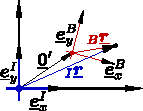
\includegraphics{./img/kosy.pdf} } \quad
	\parbox{5cm}{
		Vektor $\vec r$ zur Basis $B$:\\
		${}_B \vec r = r_x \vec e^B_x +  r_y \vec e^B_y + r_z \vec e^B_z$\\[0.5em]
		\begin{tabular}{@{}ll}
			$\vec e^B_i$ & Basisvektor von $B$ in $i$-Richtung\\
			$r_i$ & Koordinate in $i$-Richtung\\
			$r_i \vec e^B_i$ & $i$-Komponente bezüglich $B$\\
			$I$ & Basis des Inertialsystems $I$
		\end{tabular}
	}
\end{sectionbox}


\begin{sectionbox}
	\subsubsection{Ableitungsregeln ($\forall \lambda, \mu \in \mathbb R$)}
	\begin{tabular}{@{}l@{\quad}ll@{}}
		Linearität: & $(\lambda f + \mu g)' (x) = \lambda f'(x) + \mu g'(x_0)$  \\
		Produkt: & $(f \cdot g)'(x) = f'(x) g(x) + f(x) g'(x)$\\
		Quotient: & $\left(\frac{f}{g}\right)' (x) = \frac{g(x)f'(x) -f(x) g'(x)}{g(x)^2}$ \quad $\left(\frac{\text{NAZ}-\text{ZAN}}{\text{N}^2}\right)$\\
		Kettenregel & $\left( f\bigl(g(x)\bigr) \right)' = f'\bigl(g(x)\bigr) g'(x)$\\
	\end{tabular}	
\end{sectionbox}

\begin{sectionbox}
	\subsection{Integrale $\int e^x\;\mathrm dx = e^x = (e^x)'$}
	$\int_a^b f(x) \mathrm dx = F(b) - F(a)$
	\begin{tabular*}{\columnwidth}{ll}
	Partielle Integration: & $\int uw'=uw-\int u'w$\\
	Substitution: & $\int f(g(x)) g'(x)\diff x=\int f(t)\diff t$
	\end{tabular*}
	\begin{tablebox}{@{\hspace{5mm}}c@{\extracolsep\fill}c@{\extracolsep\fill}c@{\hspace{5mm}}} 
		$F(x) - C$ & $f(x)$ & $f'(x)$ \\ \cmrule
		$\frac{1}{q+1}x^{q+1}$ & $x^q$ & $qx^{q-1}$ \\[1em]
		\raisebox{-0.2em}{$\frac{2\sqrt{ax^3}}{3}$} & $\sqrt{ax}$ & \raisebox{0.2em}{$\frac{a}{2\sqrt{ax}}$}\\
		$x\ln(ax) -x$ & $\ln(ax)$ & $\textstyle \frac{1}{x}$\\
		$\frac{1}{a^2} e^{ax}(ax- 1)$ & $x \cdot e^{ax}$ & $e^{ax}(ax+1)$ \\
		$\frac{a^x}{\ln(a)}$ & $a^x$ & $a^x \ln(a)$ \\
		$-\cos(x)$ & $\sin(x)$ & $\cos(x)$\\
		$\cosh(x)$ & $\sinh(x)$ & $\cosh(x)$\\
		$-\ln |\cos(x)|$ & $\tan(x)$ & $\frac{1}{\cos^2(x)}$ \\ 
	\end{tablebox}

	\begin{tabular*}{\columnwidth}{ll}
	\multicolumn{2}{c}{$\int e^{at} \sin(bt) \diff t = e^{at} \frac{a \sin(bt) + b \cos(bt)}{a^2 + b^2}$}\\
	$\int \frac{\diff t}{\sqrt{at+b}} = \frac{2 \sqrt{at+b}}{a}$ & $\int t^2 e^{at} \diff t = \frac{(ax-1)^2+1}{a^3} e^{at}$\\
	$\int t e^{at} \diff t = \frac{at-1}{a^2} e^{at}$ & $\int x e^{ax^2} \diff x = \frac{1}{2a} e^{ax^2}$\\
	\end{tabular*}

	\subsubsection{Volumen und Oberfläche von Rotationskörpern um $x$-Achse}
	$V = \pi \int_a^b f(x)^2 \mathrm dx$ \qquad \quad $O = 2 \pi \int_a^b f(x) \sqrt{1 + f'(x)^2} \mathrm dx$
\end{sectionbox}

\begin{sectionbox}
	\subsection{Partialbruchzerlegung}
\end{sectionbox}




\begin{sectionbox}
	\subsection{Differentialoperatoren \qquad $\div(\rot \vec f) \equiv 0$}
	\begin{emphbox}
		\begin{tabular}{@{}lll}
			\textbf{Gradient} $\grad f$ & \qquad \textbf{Rotation} $\rot \vec f$\\[0.3em]
			$\nabla f = \vect{\partial_1 f \\ \svdots \\ \partial_n f }$ & \qquad $\nabla \times \vec f = \vect{\partial_y f_3 - \partial_z f_2 \\ \partial_z f_1 -\partial_x f_3 \\ \partial_x f_2 -\partial_y f_1}$\!\!\!\!\\[2.5em] 
			\textbf{Divergenz} $\div \vec f$ & \qquad \textbf{Laplace} $\Delta\, f = \Sp \ma H_f(\vec x)$\\[0.2em]
			${\displaystyle \nabla^\top \bdot \vec f = \sum\limits_{i=0}^n \frac{\partial f_i}{\partial x_i}}$ & \qquad ${\displaystyle\underset{\nabla^\top \cdot (\nabla f)}{\nabla^2 f} = \sum\limits_{i=0}^n \frac{\partial f}{\partial x_i x_i} }$\\
		\end{tabular}
	\end{emphbox}
\end{sectionbox}

% SECTION ====================================================================================
\section{Frequenzanalyse}
% ============================================================================================

\begin{sectionbox}
	\subsection{Fouriertransformation}
	\begin{emphbox}
		$\displaystyle \underset{\text{Zeitbereich}}{\large f(t)} \FT \underset{\text{Frequenzspektrum}}{\large F(\omega)} := \int\limits_{-\infty}^\infty f(t) \exp(-\i \omega t) \diff t$
	\end{emphbox} 
	Anmerkung: Es gibt unterschiedliche Normungen ($1, \frac{1}{\sqrt{2\pi}}$)\\
\end{sectionbox}



\begin{sectionbox}
	\subsection{Laplaceransformation}
	\begin{emphbox}
		$\displaystyle \underset{\text{Zeitbereich}}{\large f(t)} \LT \underset{\text{Frequenzspektrum}}{\large F(s) = \mathcal L\left(f(t)\right)} := \int\limits_{0}^\infty f(t) \exp(- s t) \diff t$
	\end{emphbox} 
\end{sectionbox}



% SECTION ====================================================================================
\section{Stochastik}
% ============================================================================================
\begin{sectionbox}
	\subsection{Kombinatorik}
	Mögliche Variationen/Kombinationen um $k$ Elemente von maximal $n$ Elementen zu wählen bzw. $k$ Elemente auf $n$ Felder zu verteilen:\\
	\begin{tablebox}{l|cc} 
		& \large Mit Reihenfolge & \large Reihenfolge egal\\ \cmrule
		%& ungleiche Elemente & gleiche Elemente \\ 
		\large Mit Wiederholung & \large $n^k$ & \Large $\binom{n+k-1}{k}$\\[0.2em]
		\large Ohne Wiederholung & \Large $\frac{n!}{(n-k)!}$ & \Large $\binom nk$\\
	\end{tablebox}
	Permutation von $n$ mit jeweils $k$ gleichen Elementen: $\frac{n!}{k_1 ! \cdot k_2 ! \cdot ...}$\\
	Binomialkoeffizient $\binom nk = \binom n{n-k} = \frac{n!}{k! \cdot (n-k)!}$\\
	$\binom n0 = 1$ \quad $\binom n1 = n$ \quad $\binom 42 = 6$ \quad $\binom 52 = 10$ \quad $\binom 62 = 15$
\end{sectionbox}





% SECTION ====================================================================================
\section{Numerische Verfahren}
% ============================================================================================
\begin{sectionbox}
	\subsection[Lineares Gleichungssystem]{Lineares Gleichungssystem $\ma A \vec x = \vec b$}
	$\ma A = \ma L \ma R$ mit $\ma L$/$\ma R$ untere/obere Dreiecksmatrix\\
	$\ma A = \ma Q \ma R$ mit $\ma Q^-1 = \ma Q^\top$\\
	$\ma A = \ma U \ma D \ma V$
\end{sectionbox}	



\begin{sectionbox}
	\subsection{Orthogonalisierungsverfahren nach Gram-Schmidt}
	Berechnet zu $n$ Vektoren $\vec v_i$ ein Orthogonalsystem $\vec b_i$\quad ($i \in [1;n])$
	\begin{equation*}
		\vec b_1 = \vec v_1 \qquad\qquad \vec b_i = \vec v_i - \sum\limits_{k=1}^{i-1} \frac{\vec b_k^\top \bdot \vec v_i}{\vec b_k^\top \bdot \vec b_k} \vec b_k
	\end{equation*}
	Erhalte Ortho\textbf{normal}system durch $\vec b_i' = \vec b_i/\norm{\vec b_i}$\\
	QR-Zerlegung: $\ma A = \ma Q \ma R$ mit $\ma Q = \big[\vec b_1', ... , \vec b_n'\big]$ \quad $\ma R = \ma Q^\top \ma A$
\end{sectionbox}

% DOCUMENT_END =================================================================
\end{document}
